\section{Illustration}

\Cref{fig:amp} plots the amplitude ratio \cref{eq:amplitude} against
$x/L$ for $\omega L/c = 7$ and several values of $\omega\tau$. The values of
$\beta L$ and $\alpha L$ follow from \cref{eq:alpha_beta}. In the undamped
case the envelope has true nodes. As damping increases, the nodes fill in and
the response approaches the decaying travelling wave $e^{-\alpha x}$.

\begin{figure}[H]
  \centering
  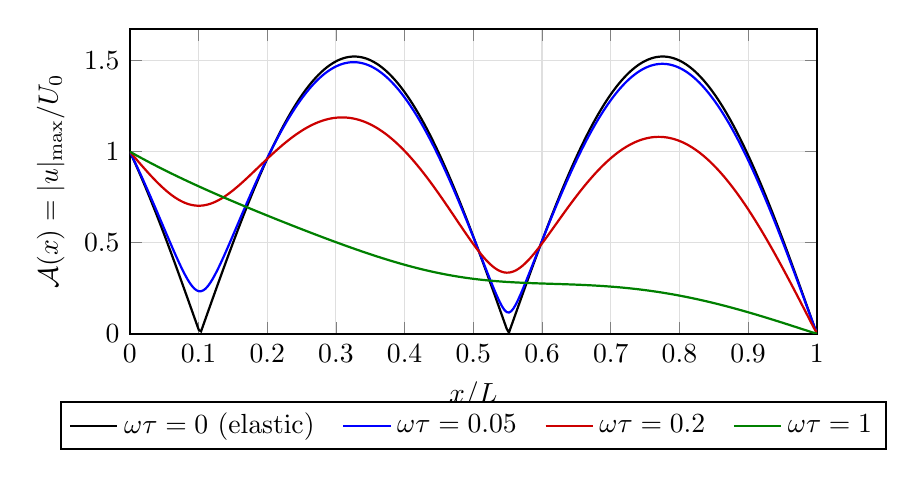
\begin{tikzpicture}
    \begin{axis}[
      width=0.85\textwidth, height=0.45\textwidth,
      xlabel={$x/L$}, ylabel={$\mathcal{A}(x) = |u|_{\max}/U_0$},
      xmin=0, xmax=1, ymin=0,
      legend style={at={(0.5,-0.22)}, anchor=north, legend columns=4, /tikz/every even column/.append style={column sep=0.8em}},
      samples=300, domain=0:1, thick,
      grid=major, grid style={gray!25},
    ]
      % omega*tau = 0:    betaL = 7.00000, alphaL = 0
      \addplot[black] {abs(sin(deg(7*(1-x))))/abs(sin(deg(7)))};
      \addlegendentry{$\omega\tau = 0$ (elastic)}
      % omega*tau = 0.05: betaL = 6.99345, alphaL = 0.17473
      \addplot[blue] {sqrt((cosh(2*0.17473*(1-x)) - cos(deg(2*6.99345*(1-x))))/(cosh(2*0.17473) - cos(deg(2*6.99345))))};
      \addlegendentry{$\omega\tau = 0.05$}
      % omega*tau = 0.2:  betaL = 6.89796, alphaL = 0.68303
      \addplot[red!80!black] {sqrt((cosh(2*0.68303*(1-x)) - cos(deg(2*6.89796*(1-x))))/(cosh(2*0.68303) - cos(deg(2*6.89796))))};
      \addlegendentry{$\omega\tau = 0.2$}
      % omega*tau = 1:    betaL = 5.43821, alphaL = 2.25258
      \addplot[green!50!black] {sqrt((cosh(2*2.25258*(1-x)) - cos(deg(2*5.43821*(1-x))))/(cosh(2*2.25258) - cos(deg(2*5.43821))))};
      \addlegendentry{$\omega\tau = 1$}
    \end{axis}
  \end{tikzpicture}
  \caption{Steady-state displacement amplitude along the rod for
    $\omega L/c = 7$. The left end is driven with amplitude $U_0$ and the right
    end is fixed.}
  \label{fig:amp}
\end{figure}
